\chapter{Digital sampling}
We studied how to reconstruct a signal starting from its sampling. We tried different sampling frequency and two different waves then using the Whittaker–Shannon formula we have reconstructed the orginal signal. 

\section{Materials}
\begin{itemize}
\item National Instruments myDAQ
\end{itemize}
\section{Experimental setup}
The waveform generator and the NI myDAQ were connected so we could have use the LabView software for aquiring the data. The sampling frequency and the number of samples were set with the software. As source signal we used a sine wave with frequency $10$ Hz and an amplitude pk-pk of $5$ V, we sampled this wave with a frequency of 5,10 and 25 Hz. Then we switched wave with a triangular one of 100 Hz and 4 V pk-pk amplitude, this last signal was sampled with a 500 Hz frequency.
\section{Data analysis}
The Whittaker–Shannon formula states that:
\[x(t) = \sum_n x_n\cdot\text{sinc}\left(\frac{t-t_n}{T}\right)\]
where $x_n$ are the data corresponding to the time $t_n$ and $T$ is the sampling period. Appling this formula to our data we obtain the following plot
\begin{figure}[H]
\centering
\begin{minipage}{.5\textwidth}
  \centering
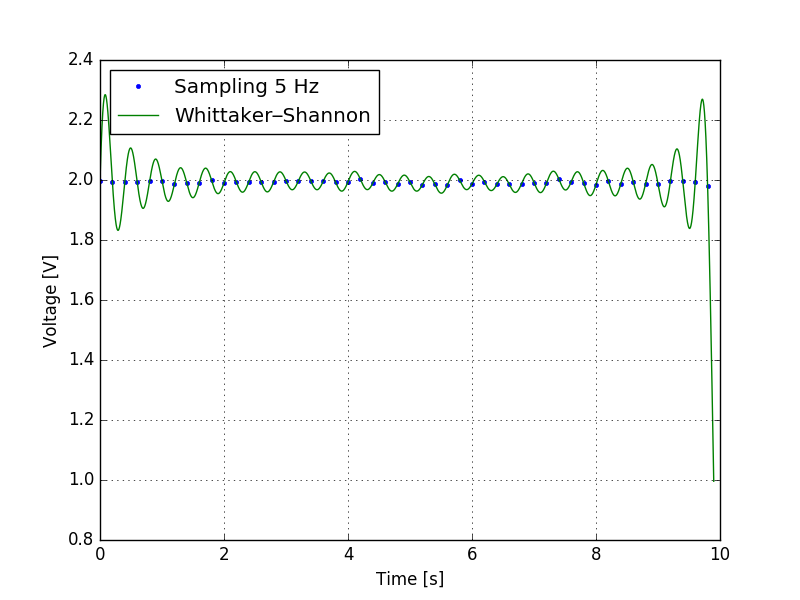
\includegraphics[width=\textwidth]{13/5Hz.png}
\caption{Sine input, sampling frequency: 5 Hz}
\end{minipage}\hfill
\begin{minipage}{.5\textwidth}
  \centering
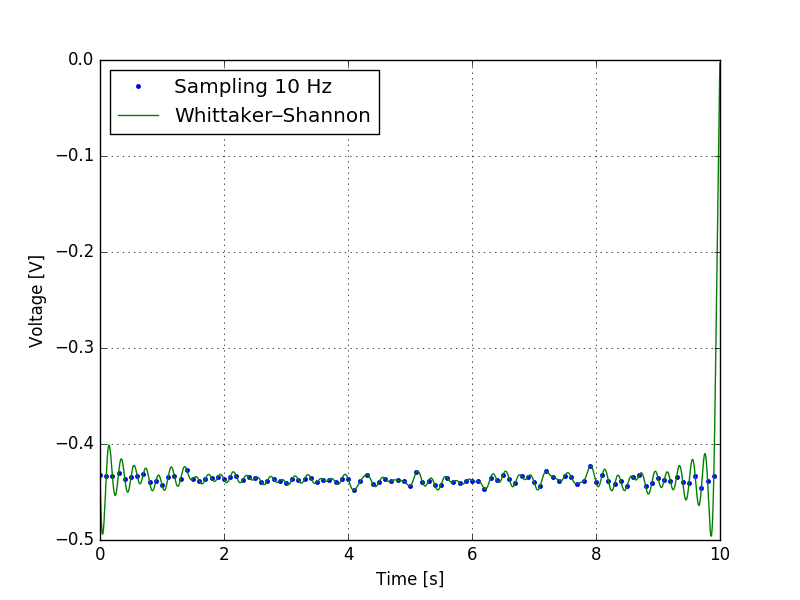
\includegraphics[width=\textwidth]{13/10Hz.png}
\caption{Sine input, sampling frequency: 10 Hz}
\end{minipage}
\end{figure}
\begin{figure}[H]
\centering
\begin{minipage}{.5\textwidth}
  \centering
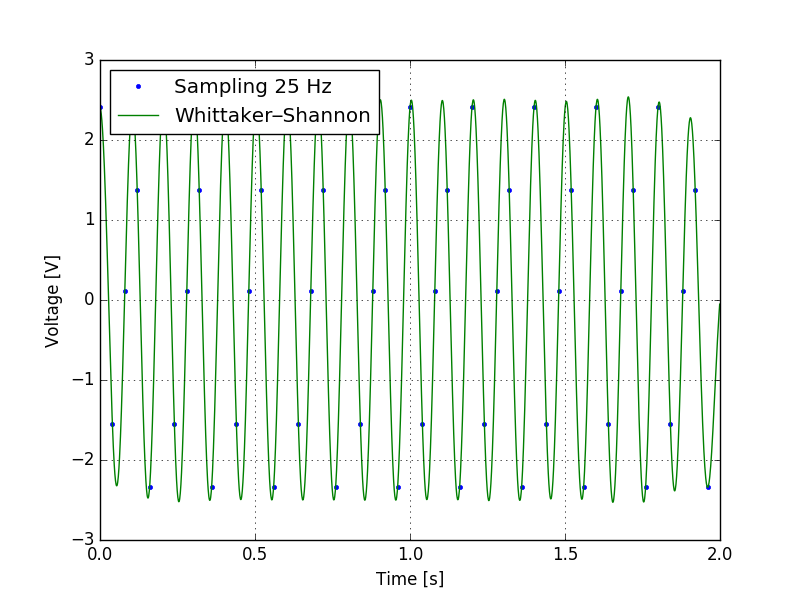
\includegraphics[width=\textwidth]{13/25Hz.png}
\caption{Sine input, sampling frequency: 25 Hz}
\end{minipage}%
\begin{minipage}{.5\textwidth}
  \centering
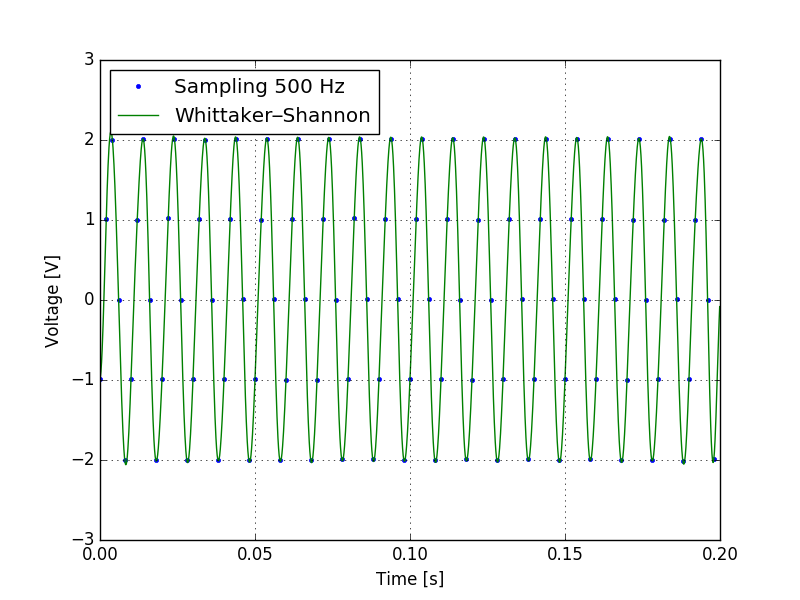
\includegraphics[width=\textwidth]{13/500Hz.png}
\caption{Triangular input, sampling frequency: 500 Hz}
\end{minipage}
\end{figure}